\documentclass{standalone}
\usepackage{tikz}
\usetikzlibrary{patterns, positioning}
\usepackage[sfdefault]{ClearSans} %% option 'sfdefault' activates Clear Sans as the default text font
\usepackage[T1]{fontenc}

\begin{document}
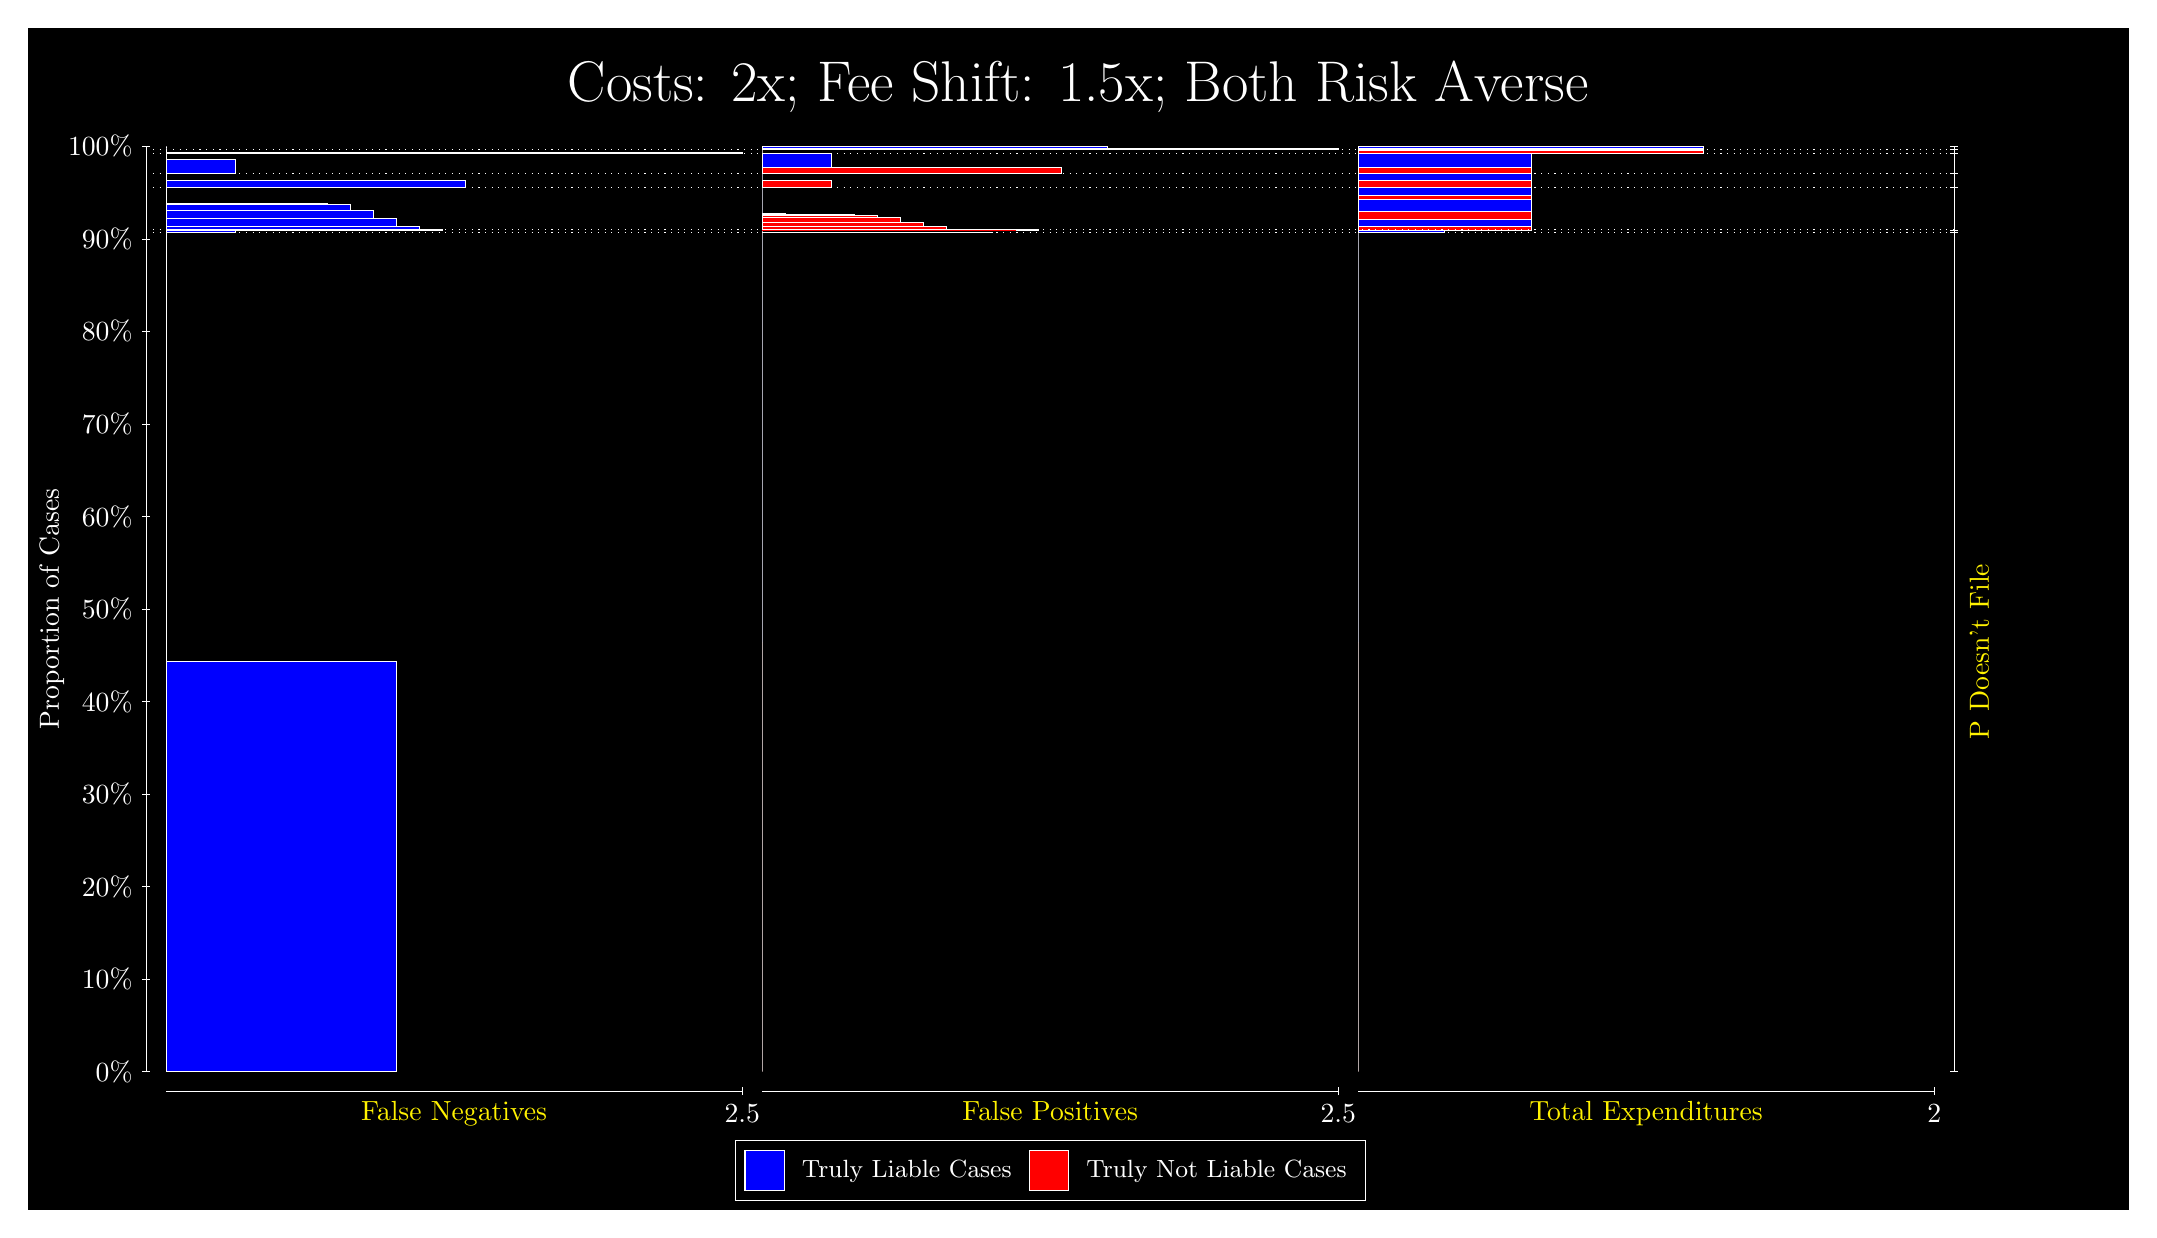
\begin{tikzpicture}
\draw[fill=black] (0,0) rectangle (26.667,15);
\draw[text=white] (0,13.5) rectangle (26.667,15) node[midway] {\huge Costs: 2x; Fee Shift: 1.5x; Both Risk Averse};
\draw[white, very thin] (1.5,1.75) -- (1.5,13.5);
\node[rotate=90, text=white, anchor=center] at (0.3, 7.625) {Proportion of Cases};
\draw[white, very thin] (1.45,1.75) -- (1.55,1.75);
\node[text=white, anchor=east] at (1.45, 1.75) {0\%};
\draw[white, very thin] (1.45,2.925) -- (1.55,2.925);
\node[text=white, anchor=east] at (1.45, 2.925) {10\%};
\draw[white, very thin] (1.45,4.1) -- (1.55,4.1);
\node[text=white, anchor=east] at (1.45, 4.1) {20\%};
\draw[white, very thin] (1.45,5.275) -- (1.55,5.275);
\node[text=white, anchor=east] at (1.45, 5.275) {30\%};
\draw[white, very thin] (1.45,6.45) -- (1.55,6.45);
\node[text=white, anchor=east] at (1.45, 6.45) {40\%};
\draw[white, very thin] (1.45,7.625) -- (1.55,7.625);
\node[text=white, anchor=east] at (1.45, 7.625) {50\%};
\draw[white, very thin] (1.45,8.8) -- (1.55,8.8);
\node[text=white, anchor=east] at (1.45, 8.8) {60\%};
\draw[white, very thin] (1.45,9.975) -- (1.55,9.975);
\node[text=white, anchor=east] at (1.45, 9.975) {70\%};
\draw[white, very thin] (1.45,11.15) -- (1.55,11.15);
\node[text=white, anchor=east] at (1.45, 11.15) {80\%};
\draw[white, very thin] (1.45,12.325) -- (1.55,12.325);
\node[text=white, anchor=east] at (1.45, 12.325) {90\%};
\draw[white, very thin] (1.45,13.5) -- (1.55,13.5);
\node[text=white, anchor=east] at (1.45, 13.5) {100\%};

\draw[white, very thin] (24.457,1.75) -- (24.457,13.5);
\draw[white, very thin] (24.407,1.75) -- (24.507,1.75);
\node[anchor=west] at (24.407, 1.75) {};
\draw[white, very thin] (24.407,12.409) -- (24.507,12.409);
\node[anchor=west] at (24.407, 12.409) {};
\draw[white, very thin] (24.407,12.44) -- (24.507,12.44);
\node[anchor=west] at (24.407, 12.44) {};
\draw[white, very thin] (24.407,12.978) -- (24.507,12.978);
\node[anchor=west] at (24.407, 12.978) {};
\draw[white, very thin] (24.407,13.157) -- (24.507,13.157);
\node[anchor=west] at (24.407, 13.157) {};
\draw[white, very thin] (24.407,13.414) -- (24.507,13.414);
\node[anchor=west] at (24.407, 13.414) {};
\draw[white, very thin] (24.407,13.463) -- (24.507,13.463);
\node[anchor=west] at (24.407, 13.463) {};
\draw[white, very thin] (24.407,13.5) -- (24.507,13.5);
\node[anchor=west] at (24.407, 13.5) {};

\draw[white, very thin, fill=blue] (1.75,1.75) rectangle (4.6775,6.9564);
\draw[white, very thin, fill=red] (1.75,6.9564) rectangle (1.75,12.409);
\draw[white, very thin, fill=blue] (1.75,12.409) rectangle (2.6283,12.436);
\draw[white, very thin, fill=red] (1.75,12.436) rectangle (1.75,12.44);
\draw[white, very thin, fill=blue] (1.75,12.44) rectangle (5.2631,12.451);
\draw[white, very thin, fill=blue] (1.75,12.451) rectangle (4.9703,12.479);
\draw[white, very thin, fill=blue] (1.75,12.479) rectangle (4.6775,12.59);
\draw[white, very thin, fill=blue] (1.75,12.59) rectangle (4.3848,12.591);
\draw[white, very thin, fill=blue] (1.75,12.591) rectangle (4.3848,12.683);
\draw[white, very thin, fill=blue] (1.75,12.683) rectangle (4.092,12.768);
\draw[white, very thin, fill=blue] (1.75,12.768) rectangle (3.7993,12.771);
\draw[white, very thin, fill=blue] (1.75,12.771) rectangle (3.5065,12.774);
\draw[white, very thin, fill=blue] (1.75,12.774) rectangle (3.2138,12.776);
\draw[white, very thin, fill=blue] (1.75,12.776) rectangle (2.921,12.777);
\draw[white, very thin, fill=red] (1.75,12.777) rectangle (1.75,12.978);
\draw[white, very thin, fill=blue] (1.75,12.978) rectangle (5.5558,13.07);
\draw[white, very thin, fill=red] (1.75,13.07) rectangle (1.75,13.157);
\draw[white, very thin, fill=blue] (1.75,13.157) rectangle (2.6283,13.332);
\draw[white, very thin, fill=red] (1.75,13.332) rectangle (1.75,13.414);
\draw[white, very thin, fill=blue] (1.75,13.414) rectangle (9.0689,13.423);
\draw[white, very thin, fill=red] (1.75,13.423) rectangle (1.75,13.463);
\draw[white, very thin, fill=red] (1.75,13.463) rectangle (1.75,13.472);
\draw[white, very thin, fill=blue] (1.75,13.472) rectangle (1.75,13.5);
\draw[white, very thin, fill=red] (9.3189,1.75) rectangle (9.3189,7.2024);
\draw[white, very thin, fill=blue] (9.3189,7.2024) rectangle (9.3189,12.409);
\draw[white, very thin, fill=red] (9.3189,12.409) rectangle (12.246,12.412);
\draw[white, very thin, fill=blue] (9.3189,12.412) rectangle (9.3189,12.44);
\draw[white, very thin, fill=red] (9.3189,12.44) rectangle (12.832,12.441);
\draw[white, very thin, fill=red] (9.3189,12.441) rectangle (12.539,12.442);
\draw[white, very thin, fill=red] (9.3189,12.442) rectangle (12.246,12.445);
\draw[white, very thin, fill=red] (9.3189,12.445) rectangle (11.954,12.448);
\draw[white, very thin, fill=red] (9.3189,12.448) rectangle (11.661,12.487);
\draw[white, very thin, fill=red] (9.3189,12.487) rectangle (11.368,12.535);
\draw[white, very thin, fill=red] (9.3189,12.535) rectangle (11.075,12.601);
\draw[white, very thin, fill=red] (9.3189,12.601) rectangle (10.783,12.624);
\draw[white, very thin, fill=red] (9.3189,12.624) rectangle (10.49,12.641);
\draw[white, very thin, fill=blue] (9.3189,12.641) rectangle (9.9044,12.642);
\draw[white, very thin, fill=blue] (9.3189,12.642) rectangle (9.6116,12.644);
\draw[white, very thin, fill=blue] (9.3189,12.644) rectangle (9.3189,12.978);
\draw[white, very thin, fill=red] (9.3189,12.978) rectangle (10.197,13.066);
\draw[white, very thin, fill=blue] (9.3189,13.066) rectangle (9.3189,13.157);
\draw[white, very thin, fill=red] (9.3189,13.157) rectangle (13.125,13.24);
\draw[white, very thin, fill=blue] (9.3189,13.24) rectangle (10.197,13.414);
\draw[white, very thin, fill=red] (9.3189,13.414) rectangle (9.3189,13.454);
\draw[white, very thin, fill=blue] (9.3189,13.454) rectangle (9.3189,13.463);
\draw[white, very thin, fill=red] (9.3189,13.463) rectangle (16.638,13.472);
\draw[white, very thin, fill=blue] (9.3189,13.472) rectangle (13.71,13.5);
\draw[white, very thin, fill=red] (16.888,1.75) rectangle (16.888,7.2024);
\draw[white, very thin, fill=blue] (16.888,7.2024) rectangle (16.888,12.409);
\draw[white, very thin, fill=red] (16.888,12.409) rectangle (17.986,12.412);
\draw[white, very thin, fill=blue] (16.888,12.412) rectangle (17.986,12.44);
\draw[white, very thin, fill=red] (16.888,12.44) rectangle (19.083,12.483);
\draw[white, very thin, fill=blue] (16.888,12.483) rectangle (19.083,12.572);
\draw[white, very thin, fill=red] (16.888,12.572) rectangle (19.083,12.679);
\draw[white, very thin, fill=blue] (16.888,12.679) rectangle (19.083,12.831);
\draw[white, very thin, fill=red] (16.888,12.831) rectangle (19.083,12.881);
\draw[white, very thin, fill=blue] (16.888,12.881) rectangle (19.083,12.978);
\draw[white, very thin, fill=red] (16.888,12.978) rectangle (19.083,13.066);
\draw[white, very thin, fill=blue] (16.888,13.066) rectangle (19.083,13.157);
\draw[white, very thin, fill=red] (16.888,13.157) rectangle (19.083,13.24);
\draw[white, very thin, fill=blue] (16.888,13.24) rectangle (19.083,13.414);
\draw[white, very thin, fill=red] (16.888,13.414) rectangle (21.279,13.454);
\draw[white, very thin, fill=blue] (16.888,13.454) rectangle (21.279,13.463);
\draw[white, very thin, fill=red] (16.888,13.463) rectangle (21.279,13.472);
\draw[white, very thin, fill=blue] (16.888,13.472) rectangle (21.279,13.5);
\draw[white, dotted] (1.5,12.409) -- (24.457,12.409);
\draw[white, dotted] (1.5,12.44) -- (24.457,12.44);
\draw[white, dotted] (1.5,12.978) -- (24.457,12.978);
\draw[white, dotted] (1.5,13.157) -- (24.457,13.157);
\draw[white, dotted] (1.5,13.414) -- (24.457,13.414);
\draw[white, dotted] (1.5,13.463) -- (24.457,13.463);
\draw[white, very thin] (1.75,1.5) -- (9.0689,1.5);
\node[text=yellow, anchor=north] at (5.4094, 1.5) {False Negatives};
\draw[white, very thin] (9.0689,1.45) -- (9.0689,1.55);
\node[text=white, anchor=north] at (9.0689, 1.45) {2.5};

\draw[white, very thin] (9.3189,1.5) -- (16.638,1.5);
\node[text=yellow, anchor=north] at (12.978, 1.5) {False Positives};
\draw[white, very thin] (16.638,1.45) -- (16.638,1.55);
\node[text=white, anchor=north] at (16.638, 1.45) {2.5};

\draw[white, very thin] (16.888,1.5) -- (24.207,1.5);
\node[text=yellow, anchor=north] at (20.547, 1.5) {Total Expenditures};
\draw[white, very thin] (24.207,1.45) -- (24.207,1.55);
\node[text=white, anchor=north] at (24.207, 1.45) {2};

\node[text=yellow, centered, rotate=90] at (24.777, 7.0794) {P Doesn't File};







\draw (12.978300999999998,1.5) node[draw=none] (baseCoordinate) {};
\begin{scope}[align=center]
        \matrix[scale=0.5, draw=white, below=0.5cm of baseCoordinate, nodes={draw}, column sep=0.1cm]{
            \node[rectangle, draw, minimum width=0.5cm, minimum height=0.5cm, fill=blue] {}; &
            \node[draw=none, font=\small, text=white] (B) {Truly Liable Cases}; &
            \node[rectangle, draw, minimum width=0.5cm, minimum height=0.5cm, fill=red] {}; &
            \node[draw=none, font=\small, text=white] (B) {Truly Not Liable Cases}; \\
            };
\end{scope}

\end{tikzpicture}
\end{document}